%% Version 4.3.2, 25 August 2014
%
%%%%%%%%%%%%%%%%%%%%%%%%%%%%%%%%%%%%%%%%%%%%%%%%%%%%%%%%%%%%%%%%%%%%%%
% Template.tex --  LaTeX-based template for submissions to the 
% American Meteorological Society
%
% Template developed by Amy Hendrickson, 2013, TeXnology Inc., 
% amyh@texnology.com, http://www.texnology.com
% following earlier work by Brian Papa, American Meteorological Society
%
% Email questions to latex@ametsoc.org.
%
%%%%%%%%%%%%%%%%%%%%%%%%%%%%%%%%%%%%%%%%%%%%%%%%%%%%%%%%%%%%%%%%%%%%%
% PREAMBLE
%%%%%%%%%%%%%%%%%%%%%%%%%%%%%%%%%%%%%%%%%%%%%%%%%%%%%%%%%%%%%%%%%%%%%

%% Start with one of the following:
% DOUBLE-SPACED VERSION FOR SUBMISSION TO THE AMS
\documentclass{ametsoc}

% TWO-COLUMN JOURNAL PAGE LAYOUT---FOR AUTHOR USE ONLY
% \documentclass[twocol]{ametsoc}

%%%%%%%%%%%%%%%%%%%%%%%%%%%%%%%%
%%% To be entered only if twocol option is used

\journal{jamc}

%  Please choose a journal abbreviation to use above from the following list:
% 
%   jamc     (Journal of Applied Meteorology and Climatology)
%   jtech     (Journal of Atmospheric and Oceanic Technology)
%   jhm      (Journal of Hydrometeorology)
%   jpo     (Journal of Physical Oceanography)
%   jas      (Journal of Atmospheric Sciences)	
%   jcli      (Journal of Climate)
%   mwr      (Monthly Weather Review)
%   wcas      (Weather, Climate, and Society)
%   waf       (Weather and Forecasting)
%   bams (Bulletin of the American Meteorological Society)
%   ei    (Earth Interactions)

%%%%%%%%%%%%%%%%%%%%%%%%%%%%%%%%
% Citations should be of the form ``author year''  not ``author, year''
\bibpunct{(}{)}{;}{a}{}{,}

%%%%%%%%%%%%%%%%%%%%%%%%%%%%%%%%

%%% To be entered by author:

%% May use \\ to break lines in title:

\title{Sensitivity of bow-echo forecasts to ensemble and model configuration}

%%% Enter authors' names, as you see in this example:
%%% Use \correspondingauthor{} and \thanks{Current Affiliation:...}
%%% immediately following the appropriate author.
%%%
%%% Note that the \correspondingauthor{} command is NECESSARY.
%%% The \thanks{} commands are OPTIONAL.

    %\authors{Author One\correspondingauthor{Author One, 
    % American Meteorological Society, 
    % 45 Beacon St., Boston, MA 02108.}
% and Author Two\thanks{Current affiliation: American Meteorological Society, 
    % 45 Beacon St., Boston, MA 02108.}}

\authors{John Lawson \correspondingauthor{Dept., Institution, Address, City, State/Country.}}

%% Follow this form:
    % \affiliation{American Meteorological Society, 
    % Boston, Massachusetts.}

\affiliation{Department of Geological and Atmospheric Sciences, Iowa State University, United States of America.}

%% Follow this form:
    %\email{latex@ametsoc.org}

\email{johnroblawson@gmail.com}

%% If appropriate, add additional authors, different affiliations:
    %\extraauthor{Extra Author}
    %\extraaffil{Affiliation, City, State/Province, Country}

\extraauthor{William A. Gallus, Jr.}
%\extraaffil{}

%% May repeat for a additional authors/affiliations:

%\extraauthor{}
%\extraaffil{}

%%%%%%%%%%%%%%%%%%%%%%%%%%%%%%%%%
%%% EXTRA PACKAGES/SHORTCUTS %%%%
% DEFINITIONS 
\def\gefs{\mbox{GEFS/R2}} %Avoid line breaks
\def\approx{$\sim$}

%%%%%%%%%%%%%%%%%%%%%%%%%%%%%%%%%%%%%%%%%%%%%%%%%%%%%%%%%%%%%%%%%%%%%
% ABSTRACT
%
% Enter your abstract here
% Abstracts should not exceed 250 words in length!
%
% For BAMS authors only: If your article requires a Capsule Summary, please place the capsule text at the end of your abstract
% and identify it as the capsule. Example: This is the end of the abstract. (Capsule Summary) This is the capsule summary. 

\abstract{Bow-echo structures, both embedded within quasi-linear convective systems and as singular systems, are often poorly forecast within deterministic numerical weather prediction model simulations. However, the spread of bow-echo structures within an ensemble of model runs is not known. This study assesses the inter-ensemble-member sensitivity of the structures' simulated reflectivity and radius of curvature to the following: perturbations in initial conditions using a global dataset; different microphysical schemes; and in response to the use of a stochastic kinetic-energy backscatter (SKEB) scheme. It is found that the ensemble spread decreases, respectively, through the three aforementioned ensemble types. Interestingly, a poor deterministic forecast using a given microphysical scheme and a given set of initial conditions can be somewhat improved in some SKEB ensemble members, suggesting that model error needs to be better accounted for when forecasting these mesoscale phenomena, and that one-shot evaluations of parameterization schemes are dangerous.}

\begin{document}

%% Necessary!
\maketitle


%%%%%%%%%%%%%%%%%%%%%%%%%%%%%%%%%%%%%%%%%%%%%%%%%%%%%%%%%%%%%%%%%%%%%
% MAIN BODY OF PAPER
%%%%%%%%%%%%%%%%%%%%%%%%%%%%%%%%%%%%%%%%%%%%%%%%%%%%%%%%%%%%%%%%%%%%%
\sloppy 
\section{Introduction}

Mesoscale convective systems (MCSs) are groups of thunderstorms of length $O$(100\,km) in at least one direction \citep{American_Meteorological_Society2014-mi}. These predominantly summertime systems provide the Great Plains of the United States with much of their warm-season rainfall \citep{Fritsch1986-xs}. A subset of these MCSs that contain bowing features, however, bring the risks of damaging winds, 1--2\,in hail, and flash flooding \citep{Gallus2008-bm}. Conspicuous by their convex structure in radar reflectivity (Fig.~\ref{fig:verif_4panel}), bow echoes and line-echo wave patterns (LEWPs) are associated with some of the strongest wind events in the Plains, sometimes meeting derecho (damaging straight-line wind) criteria \citep{Johns1987-qj}. A bowing structure develops when stratiform precipitation behind a quasi-linear convective system (QLCS) lowers a rear-inflow jet through evaporative cooling and consequent negative buoyancy \citep{Markowski2010-xi}. This jet advects the cold pool faster in its centre, creating the distinctive bowing shape. 

%(Gallus ref to show BE wind reports; BE paper to talk about theoretical reason, downbursts etc)
Bow echoes in particular can be poorly simulated by numerical model forecasts \citep{Keene2013-df;Snively2014-pr}. Snively and Gallus found weaker 0--6\,km shear and higher potential temperatures aloft were responsible for deterministic forecast failures in numerical simulations. They also surmised that simulations involving elevated convection may have been amongst the worst. Interestingly, the study found evidence that convective morphology was not substantially sensitive to mesoscale meteorological parameters. In two studies, Adams-Selin and co-authors found that performance of numerical simulations, both idealised \citeyearpar{Adams-Selin2013-ca} and real-life \citeyearpar{Adams-Selin2013-om}, were acutely sensitive to the chosen parameterisation. Specifically, when graupel hydrometeors were simulated as lighter and greater in number, they resulted in a stronger cold pool and rear-inflow jet, and hence the bowing initiated earlier. The chosen parameterisation scheme also strongly affected pertinent forecast parameters such as precipitation amount, system speed, wind gusts, and areal coverage. The issue with these conclusions is their lack of generality to other events, including variations in synoptic regime, the initial condition dataset, and poor sampling of the model attractor (or model climate) via use of a deterministic approach. While computational and time limitations preclude in-depth analysis repeated for many cases, these methodological shortcomings nonetheless motivate a more general ensemble approach with cases in different synoptic regimes.

While numerical weather prediction (NWP) continues its march towards explicit resolution of smaller and smaller convective features, there are a number of obstacles en route that may inhibit, or even preclude, successful numerical forecasts of bow echoes. Our computer models are incomplete and imperfect: while smaller phenomena are resolved explicitly by ever-decreasing grid spacings, there will always be a scale at which chaotic, non-linear processes are implicitly resolved, or parameterised. Parameterisation is currently used in operational NWP models, such as the North American Mesoscale (NAM) model and the Global Forecasting System (GFS), to capture the planetary boundary layer (PBL), surface radiation, cloud microphysics, and so on. The ‘spread’ of parameterisation schemes developed by different institutions and researchers is not controlled, and as such, biases in each scheme can constructively or destructively interfere within a forecast run, without {\it a priori} knowledge of the impact on the forecast compared to {\it a posteriori} verification from radar reflectivity observations. For example, Adams-Selin and coauthors \citeyearpar{Adams-Selin2013-om} found bow-echo forecasts to vary substantially when solely changing the microphysical parameterisation. In their study, the authors called for schemes of opposing biases to be combined in operational mixed-physics ensemble systems; however, we cannot be sure that the biases shown in one study can apply generally to all regions, synoptic regimes, seasons, years, etc. Likewise, \citet{Berner2011-pd} trained their mixed-physics models over a number of months to determine the optimal configuration for spread and skill. This is, of course, not a practical or general approach for operational centres to endorse long-term, when one considers the training sensitivity to many factors.

In addition to model error, the atmosphere as a partly chaotic system is sensitive to initial condition error \citep{Lorenz1969-xw}. As such, Lorenz suggested a theoretical limit of predictability, estimated when assuming purely chaotic (turbulent) flow. On scales of 10\,km, Lorenz estimated predictability to be limited to 1--2\,h. Fortunately from a forecasting standpoint, it is evident in forecast models that the atmosphere has inherent predictability at the mesoscale longer than that proposed by Lorenz. This may be due to known forcings --- high terrain, synoptic-scale fronts (e.g., \citealt{Anthes1985-ga}) --- and stable mechanisms that locally limit error growth, such as supercells \citep{Lilly1990-vs}, and in confluent, weak flow \citep{Oortwijn1998-rk}. Palmer and coauthors \citeyearpar{Palmer2014} suggest that skillful forecasts past Lorenzian (\approx 2 week) timescale may be due to the intermittent nature of chaos in the atmosphere (i.e., regime dependency). In addition, they argue that Lorenz's overly pessimistic estimates are due to the overly simplistic nature of the Lorenz-63 system \citep{Lorenz1963-zy}. Unfortunately for MCS forecasts, moist convection is very destructive to predictability \citep{Zhang2003-sa}, even affecting global-model forecasts of blocking patterns in Europe at the medium-range \citep{Rodwell2013-jo}. In addition, diagnosis of substantially damaging initial-condition error is fraught with difficulty due to both up- and downscale growth of errors (\citealt{Durran-2014-qf}, and references therein). Notably, \citet{Kuhnlein2014-ys} showed that global-model initial-condition perturbations may not capture the variance in convective scales, which impacts particularly the first six hours of a forecast time.

% Palmer et al. 2014 "The Real Butterfly Effect"
%\citep{Palmer2014-cv}

To address these problems and better sample the spectrum of possible outcomes of the model atmosphere, many forecast centres use a number of different numerical simulations (ensemble forecasts). There are different ways of creating members that differ from their control: through mixed-parameterisation configurations; through perturbed initial conditions; etc. Recently, studies have yielded a method to return kinetic energy erroneously dissipated in the model between the resolved and unresolved scales to better account for model error. This so-called stochastic kinetic energy backscatter (SKEB) scheme has been shown to improve ensemble spread and ultimately provide a more skillful ensemble mean than a mixed-physics approach, except at the surface \citep{Berner2011-pd}. Furthermore, when a SKEB scheme was combined in that study with a mixed-parameterisation configuration, performance was even better. As parameterisations are deterministic in nature, a stochastic approach is potentially a better way to account for model error \citep{Palmer2001-hh}. Ensemble forecasts are not only useful for operational centres, but can provide a larger corpus of `alternative realities' in which to seek sensitivity of atmospheric phenomena \citep{Hanley2013-ch}. Hence, it seems prudent to approach ensemble creation through numerous methods, with the caveat that not all methods can rigorously measure predictability in its purest sense. 

% This paper will provide an initial foray into the following questions: 1) in terms of convective mode and the presence of bowing, is the quality of a (deterministic, ensemble) forecast systematically sensitive to the larger-scale setting? 2) When a NWP model forced by archived (re)forecast data incorrectly resolves the mode of a system, is this poor performance more related to model error or to initial conditions? Of course, these questions will not be answered in sufficient depth at this stage, but the preliminary results may provide a foundation for further investigation.

% Weisman and Davis 1998: "subsystem-scale vortices"
As a final note on nomenclature, this study will borrow the dichotomous categorisation of derechoes in \citet{Johns1987-qj} by dividing bowing features into two groups: those that appear multiple times along a QLCS, typically in parallel with a front (serial bow echoes, Fig.~\ref{fig:verif_4panel}b,c), and those that are less-strongly forced by a large-scale boundary, whose bowing radius of curvature is similar to the size of the system itself (progressive bow echoes, Fig.~\ref{fig:verif_4panel}a,d). This is motivated by the wish to concentrate on the potentially flexible criteria of radar reflectivity signatures, rather than strict (and more arbitrary) surface-wind definitions of a derecho. Furthermore, not all bow echoes are derechoes, and {\it vice versa}.
% progressive type associated with warm-front perpendicular to system?

\section{Data and Methods}
The study focuses on four cases (Fig.~\ref{fig:verif_4panel}): (a) a progressive bow echo, 26--27 May 2006; (b) a serial bow echo, 10--11 September 2009; (c) a serial bow echo, 19--20 May 2011; and (d) a progressive bow echo, 15--16 August. Each case may be referenced in the following sections in short by its letter: Case A, Case B, and so on.

All numerical simulations were performed on the same supercomputer system to avoid introduction of rounding-error contamination. The simulations were performed with version 3.5 of the Weather Research and Forecasting model (WRF;\citealt{Skamarock2008-yw}), using the Advanced Research WRF dynamical core. The control parameterisation configuration (Table~\ref{tab:WRFconfig}) was chosen primarily for stability, due to the large number of ensemble runs required with this (or most of this) control configuration. The control microphysical parameterisation (Thompson) was also selected due to good performance in similar studies (Brian Squitieri, personal communication). The constant domain size is 451 by 451 points with grid spacing $\Delta x$ set at 3\,km. The domain location varied depending on the case study; each location is shown in Figure~\ref{fig:domains}. The timestep was six seconds (i.e. $2\, \Delta x$). Fifty vertical levels were specified manually to better resolve the PBL, as found in similar studies (David Jahn and Brian Squitieri, personal communication). 

Depending on the ensemble experiment, initial and boundary conditions were provided by one member of the 11-member Global Ensemble Forecast System Reforecast dataset (\gefs), or the North American Mesoscale (NAM) archive analyses. As the \gefs{} dataset does not contain sufficient resolution in soil layers for the WRF to run as-is, Global Forecast System analyses of soil temperature and moisture were prescribed for each batch of initial and boundary conditions (see \citealt{Lawson2013-az} for further information on this method). While there is no doubt that small changes in variables such as soil temperature can affect convective initiation \citep{Clark1995-yy}, the absence of perturbations in soil variables is not likely to affect any relativistic conclusions through this method. Boundary conditions were specified every three hours. All runs were initialised on 0000 UTC on the first day of the case study, and ran for 36 hours (39 hours for Case B) to (a) allow mesoscale systems to develop in good time, (b) to allow perturbations between ensemble members to grow large enough to observe easily, but not so large that the timescale of interest was beyond the theoretical predictability limit for meso-$\alpha$-scale motion, and (c) to allow use of the once-daily \gefs{} data.

Eleven-member WRF--\gefs{} ensembles were created by running WRF eleven times, each with a different set of initial and boundary conditions from the \gefs{} dataset, with the control configuration (Table~\ref{tab:WRFconfig}. The \gefs{} control member and ten perturbation members were all used for both inspection of atmospheric variables and computation of error growth. This ensemble setup is hereby termed \textbf{ICBC}. Ensembles were also created by varying the microphysical scheme (termed \textbf{MXMP}), but holding all else constant (and selecting a constant ICBC input data set). The 11 microphysical schemes (that supplement the control scheme, Thompson) used here are detailed in Table~\ref{tab:MPs}. The schemes were chosen to mirror a similar study by \citet{Adams-Selin2013-om}. In their method, the fall speed of hail was modified in the WRF source code, so that a parameterisation could become `hail-like' or `graupel-like'. An identical method has been used in this study for the WSM6, WDM6, and Morrison schemes (Adams-Selin, personal communication), to improve the sampling of `parameterisation space'. As a caveat to the MXMP method, each member is not {\it a priori} equally as likely to ultimately simulate the `correct' solution in the same sense as a controlled ICBC ensemble. Hence, this ensemble method is technically a sensitivity study, and as such does not as rigorously measure predictability. However, it can offer insight into performance of each parameterisation scheme. To more rigorously sample the model error, a final ensemble method is used: a SKEB scheme \citep{Berner2011-pd} accounts for kinetic energy lost between resolved and unresolved scales by randomly \footnote{The `randomness' is via a seed integer specified in the WRF namelist. Hence unlimited independent ensemble members can be created by changing this value.} `injecting' kinetic energy back into the wind field. This ensemble method, termed \textbf{STCH}, requires a prescribed ICBC dataset and MXMP parameterisation. Overall, notwithstanding the previous caveat about the lack of rigour in use of MXMP members to assess predictability, this methodology is summarised in Figure~\ref{fig:method}. While this schematic follows the selection of the best-performing members to assess the stability of a ICBC ensemble member solution, it can also be used to see if a poorly performing member is a `one-off', or is a representative sample of that particular model climate. The assumption that spread decreases in ICBC, MXMP, and STCH ensembles, respectively, is supported by experimental results, as follows in the next section.

To track error growth through the ensemble domains, difference total energy (DTE) at a given timestep was calculated in a similar way to \citet{Tan2004-ss}, as follows:

\begin{align}
\textrm{DTE} = \frac{1}{2} \sum (U_{ijk}'^2 + V_{ijk}'^2 + \kappa \, T_{ijk}'^2) 
\end{align}

\noindent where $\kappa$ here \footnote{DTE has been formulated using this constant value, or as in \citet{Tan2004-ss}, via use of a reference temperature. Nonetheless, a constant is used here without ill-effect; the value of DTE in this study is in relative comparison between ensemble methods.} is 0.286, and $U'$, $V'$, and $T'$ are the differences in zonal wind, meridional wind, and potential temperature, respectively, at every grid point ($i$,$j$,$k$) between two ensemble members. This is summed over all three dimensions to create a time series, or solely in height to create a latitude--longitude cross-section. In this study, for each ensemble, $n$ sets of differences were calculated between all permutations of the $N$ ensemble members without repetition, where $n = \frac{N}{N-1} + 1$. 

\section{Error growth in all four cases}

Figure~\ref{fig:verif_4panel} shows characteristic radar reflectivity signatures of the four MCS cases. Due to space limitations, model output for Cases A--C will be described briefly rather than shown due to the large (44) amount of ensemble members. A descriptive, subjective summary is found in Table~\ref{tab:summary}.

The progressive bow echo of 26--27 May 2006 (Case A, Fig.~\ref{fig:verif_4panel}a) has been covered in more detail in \citet{Snively2014-pr}, where the authors found WRF runs forced by both NAM and GFS forecast data to incorrectly reproduce the convective mode of the MCS. They also found little sensitivity to microphysical schemes. An ICBC experiment of this event (not shown) found even poorer performance when forced with \gefs{} conditions; a NAM-forced run was a little more successful, and lays the foundation for further study (see Section~\ref{sec:futurework}). The serial bow echo of 10--11 September 2009 (Case B) contained LEWP-like features embedded along its (QLCS) length, particularly around 0800 UTC on the 11th (Fig.~\ref{fig:verif_2009}). This QLCS was associated with a cold front. Case C is a dramatic example of a serial bow echo that spawned multiple tornadoes and other severe weather on 19--20 April 2011. Finally, a progressive bow echo brought damaging wind and hail to Kansas, Oklahoma, and Texas on 15--16 August 2013. This case (D) will be the subject of a more in-depth subsection later in this paper.

In summary: Case A emphatically did not correctly simulate convection; Case B struggled to correctly simulate the QLCS and its orientation, and bowing along the line was intermittent across members, but it was generally successful; Case C did not simulate the dramatic bowing seen in observations, and only some members formed an unbroken line of convection, others simulating more discrete cells; finally, Case D was most successful, with a progressive bow echo simulated in almost all cases, timing and location errors notwithstanding.

Figure~\ref{fig:DTE_ICBC} shows the time series of DTE summed over all three spatial dimensions at each time, for the ICBC experiment from the four cases in this study. Each plotted line represents the average DTE growth of all eleven (ten perturbation and one control) ensemble-member permutations (without repetition) that involve that member. The black line is then the average of these averages. Absolute DTE values cannot be compared between cases, as the value is highly dependent on the geographical region, mesoscale environment, etc. However, it is useful to look at relative growth rates, which can be generally contrasted between cases. For instance, Case A does not experience rapid (quasi-exponential) DTE growth until around the time of maximum solar insolation on 26 May. This may be related to the onset of cellular convection at this time; before this (when DTE growth is limited), despite large areas of radar reflectivity across the domain (not shown), the mode is larger scale (and potentially less destructive in terms of predictability). Conversely, it could simply be due to the limited small-scale variance seen in the initial six hours of a numerical simulation forced by global data with large-scale perturbations \citep{Kuhnlein2014-ys}. Interestingly, despite very poor reflectivity simulation in the ICBC ensemble, error growth is comparable in rate and magnitude to the other, better-simulated progressive bow echo (Fig.~\ref{fig:DTE_ICBC}d).

Case B, in contrast, sees a slow quasi-exponential growth rate. As errors may saturate and cascade upscale faster at smaller scales (not tested here), the limited DTE growth earlier in the period in Case B may be related to a strong coupling with the synoptic-scale cold front. On the other hand, the orientation of the QLCS varies quite drastically at the time of bowing (around 0800 UTC), perhaps related to the position of the cold front, and we may expect these large-scale errors to propogate downscale (and be reflected in the DTE data), as noted by \citet{Durran_undated-qf} (in press). To diagnose whether this explains the delay of large DTE growth as seen in the other three cases in Fig.~\ref{fig:DTE_ICBC}, a spectral analysis amongst other things is required (see Section~\ref{sec:futurework}).

The magnitude of DTE in Case C is around 50\% larger (note the different y-axis scale in Figure), likely related to the large scale of the QLCS and the strong convection (compare Fig.~\ref{fig:verif_4panel}c with panels a,b,d). The growth rate pattern by eye appears to be a hybrid of Case A (early- then late-period convection) and Case B (potential strong coupling with large-scale boundary). With limited data, we may conjecture this is a reflection of multiple embedded small-scale bowing features within a larger-scale QLCS.

Finally, Case D shows a strong bimodal structure of DTE, with maxima around midnight local time for both days (around 6 and 30 forecast hours). This is likely related to vigorous convection in these periods. More interesting is the intermediate recovery. This may simply be regression to the mean; i.e., the rapid growth of DTE within areas of cellular convection ceases and a more typical environmental balance of variables is assumed. It could also be related to the movement of thunderstorms outside the domain, and advection of more tranquil air into the domain. However, it could be related to the (presumed) nocturnal low-level jet (NLLJ) that is often instrumental in nocturnal convection in the Great Plains. The dependence of the NLLJ on the Coriolis parameter and high terrain (i.e., known forcings) may converge ensemble solutions towards a model attractor. Alternatively, divergent flow within the NLLJ may separate parcel pairs (i.e., increase the Lyanpunov exponent) and hence decrease predictability (similarly, convergent flow in the nose of the NLLJ may increase predictability). The relationship of the NLLJ to theoretical predictability is unfortunately discussed little in the literature (see Section~\ref{sec:futurework}).

\section{Comparison of two progressive bow echoes}~\ref{sec:prog}

\section{Comparison of two serial bow echoes~\ref{sec:serial}

\section{Stability of a deterministic simulation}
The focus will now be on the case of 15--16 August 2013, to better evaluate its predictability, to observe the growth of errors, and to assess the performance of the ensembles. Specifically: is the good performance of the ICBC experiment related to fortuitous selection of microphysics and other aspects of the model configuration? (Interestingly, the reforecast-forced ICBC runs outperformed the NAM-analysis-forced run.) To address this, DTE will be assessed, first by integrating vertically to get a spacial sense of its distribution, then via MXMP and STCH experiments based on the best-performing set of initial and boundary conditions (p09, not shown). Figure~\ref{fig:DTE_2D} shows vertically-integrated DTE evolving through Case D at selected time, and for reference, Fig.~\ref{fig:verif} displays the composite radar reflectivity observed at the same times. 

At the first time (0300 UTC on the 15th, Fig~\ref{fig:DTE_1} and Fig~\ref{fig:DTE_1v}), three hours into the simulation, the spread is larger in two general areas: (1) locations with moist convective activity (seen in simulated radar reflectivity), where DTE growth is much larger \citep{Zhang2003-sa}, and (2) along the surface-pressure trough (not shown) running west--east in Nebraska. Over the next six hours, convection dominates the areas of rapid DTE growth (cf.\ Fig~\ref{fig:DTE_2013}). The arc of locally high DTE in southwest Nebraska to northeast Colorado (0900 UTC on the 15th, Fig~\ref{fig:DTE_2} and Fig~\ref{fig:DTE_2v}) appears to be related to discrepancies between members in simulating an outflow boundary, which is apparent in individual ensemble members' surface pressure fields (not shown). This area is also associated with a developing mesoscale convective vortex (MCV) as noted by Storm Prediction Center (SPC) mesoscale discussions. This MCV moves east-southeast over the next nine hours; at (1800 UTC on the 15th (Fig~\ref{fig:DTE_3} and Fig~\ref{fig:DTE_3v})), note the increasing homogeneity in the DTE field as convection dissipates (and again, cf.\ Fig~\ref{fig:DTE_2013}). Yet the local maximum of DTE associated with the MCV stands out from this background field; at 1800 UTC, convection initiates in the region of the MCV both in observations and most simulations (not shown). The next twelve hours summarise the essence of chaos theory: these small variations in initial location and timing of convective initiation, related to differences in the structure of the MCV between ensemble members, grow to become large DTE values as almost all members generate a progressive bow echo that moves southward through Kansas and Oklahoma (0600 UTC on the 16th, Fig~\ref{fig:DTE_4} and Fig~\ref{fig:DTE_4v}), but all in different locations with variations in bowing structure (e.g., Fig.~\ref{fig:CaseD_ICBC} three hours earlier). The mode solution appears to be highly predictable (conceptually, a large basin of attraction), even if the location and specifics of the bowing is not.

Next, the stability of this control simulation is assessed by running a MXMP ensemble with the `best' initial conditions (subjectively chosen as p09). Figure~\ref{fig:DTE_MXMP} shows the average DTE growth for each parameterisation permutation pair \footnote{Say that fast three times}. Figure~\ref{fig:CaseD_MXMP}, to aid physical interpretation, is the postage-stamp plot of composite reflectivity found in each member. We find both outputs support the assumption in the methodology that spread is reduced (at least, at these forecast ranges) when using MXMP rather than ICBC ensembles. Note this does not necessarily equate to a more skillful ensemble-mean forecast. The composite reflectivity plots show much less variation in location, but still variation in structure. When we delve further, and run a STCH ensemble based on the successful control microphysics, and the same p09 initial and boundary conditions, we find even greater convergence of solutions towards a bow echo that is similar to verification (Fig.~\ref{fig:CaseD_STCH}). Again in support of the methodology, error growth is lower still (Figs.~\ref{fig:DTE_STCH_T} and ~\ref{fig:DTE_STCH_M}). Interestingly, the `bad' microphysics scheme (deemed to be Morrison (hail-like)) was more successful in some STCH members, showing again the danger of using one deterministic forecast to make conclusions about a model scheme. The decreased DTE magnitude in STCH ensembles is related to even more spatial agreement, and slightly less variation in structure (but still substantial enough to warrant further investigation). Plotting maximum 10-m wind over the period of the bow echo (not shown) finds this variation not merely superficial, but reflected in surface wind potentially associated with downbursts within the bow echo. While this is an initial foray, future work will include investigate the physical background to the variations of the STCH members in this ensemble.

\section{Summary and Future Work}  \label{sec:futurework}
To simply attribute bow-echo simulation failure on deficiencies with a microphysical parameterisation is dangerous: the concluded sensitivity may itself be sensitive to initial and boundary conditions (the synoptic regime, time of year, etc.) and model configuration (other parameterisations, domain size, etc.). To account for these two sensitivities, ICBC and STCH ensembles, respectively, were run to assess the stability of a `good' forecast. A MXMP experiment allows comparison with other studies, and can lay the groundwork to better address the physical reasons for model error in future. In particular, Skew-Ts and cross-sections for members that are good or bad within e.g. the STCH ensemble may shed light on physical processes responsible for good and bad simulations.

Preliminary findings include:

\begin{itemize}
\item The poor performance of NWP models in Case A seen in \citet{Snively2014-pr} is not solved by varying initial conditions. This might be indictive of a trigger so small that available models cannot create perturbations on a scale small enough to recreate the bow echo evolution in at least one member.
\item Case D appears to be a highly predictable case. Considering the opposite in Case A, this suggests that poor NWP model performance is not necessarily related to the bow-echo sub-type morphology.
\item Both Cases B and C contain much variation in LEWP-type bowing structures. Case B forecasts varied more in QLCS orientation, while Case C forecasts varied in the production of slabular versus cellular convection. No members in Case C managed to recreate the dramatically large radii of curvature seem in the LEWP-type bowing features.
\item Spread in this study decreases between ensemble members in ICBC, MXMP, STCH, in descending order.
\item A poorly performing microphyiscal scheme may not be any worse than others when used with SKEB perturbations (i.e., the poor solution is not stable).
\end{itemize}

In light of the recategorisation of bow echoes into progressive and serial sub-types, a similar reclassification of cases in \citet{Snively2014-pr} may reveal a tendency for one type over the other to be associated with poor skill scores assessed in that study. 

To further this study's methodology, MXMP and STCH ensembles will be conducted for the other three cases, and spectral analysis will be performed on DTE data to somewhat normalise error growth by event, and to diagnose the source of errors at an early stage. Finally, additional topics may include the stochastic parameterisation for hail/graupel to better reflect uncertainty in the atmospheric variables; an investigation into the predictability of the NLLJ and potential impact on error growth within mesoscale systems in the Great Plains; and whether the conceptual basin of attraction for convective mode is fractal-like, with very unstable solutions, and if so, whether this basin structure is sensitive to an atmospheric tuning parameter akin to the control parameter in chaotic dynamical systems $k$ (e.g., \citealt{Williams1997-yg}, p.161).

\begin{acknowledgment} 
The author thanks Rachael Adams-Selin and her colleagues for supplying the Fortran modifications and advice relating to the microphysical schemes.
\end{acknowledgment}

%% In all cases, if there is only one entry of this type within
%% the higher level heading, use the star form: 
%%
% \section{Section title}
% \subsection*{subsection}
% text...
% \section{Section title}

%vs

% \section{Section title}
% \subsection{subsection one}
% text...
% \subsection{subsection two}
% \section{Section title}

%%%
% \section{First primary heading}

% \subsection{First secondary heading}

% \subsubsection{First tertiary heading}

% \paragraph{First quaternary heading}

%%%%%%%%%%%%%%%%%%%%%%%%%%%%%%%%%%%%%%%%%%%%%%%%%%%%%%%%%%%%%%%%%%%%%
% ACKNOWLEDGMENTS
%%%%%%%%%%%%%%%%%%%%%%%%%%%%%%%%%%%%%%%%%%%%%%%%%%%%%%%%%%%%%%%%%%%%%
%
\acknowledgments
Start acknowledgments here.

%%%%%%%%%%%%%%%%%%%%%%%%%%%%%%%%%%%%%%%%%%%%%%%%%%%%%%%%%%%%%%%%%%%%%
% APPENDIXES
%%%%%%%%%%%%%%%%%%%%%%%%%%%%%%%%%%%%%%%%%%%%%%%%%%%%%%%%%%%%%%%%%%%%%
%
% Use \appendix if there is only one appendix.
%\appendix

% Use \appendix[A], \appendix}[B], if you have multiple appendixes.
%\appendix[A]

%% Appendix title is necessary! For appendix title:
%\appendixtitle{}

%%% Appendix section numbering (note, skip \section and begin with \subsection)
% \subsection{First primary heading}

% \subsubsection{First secondary heading}

% \paragraph{First tertiary heading}

%% Important!
%\appendcaption{<appendix letter and number>}{<caption>} 
%must be used for figures and tables in appendixes, e.g.,
%
%\begin{figure}
%\noindent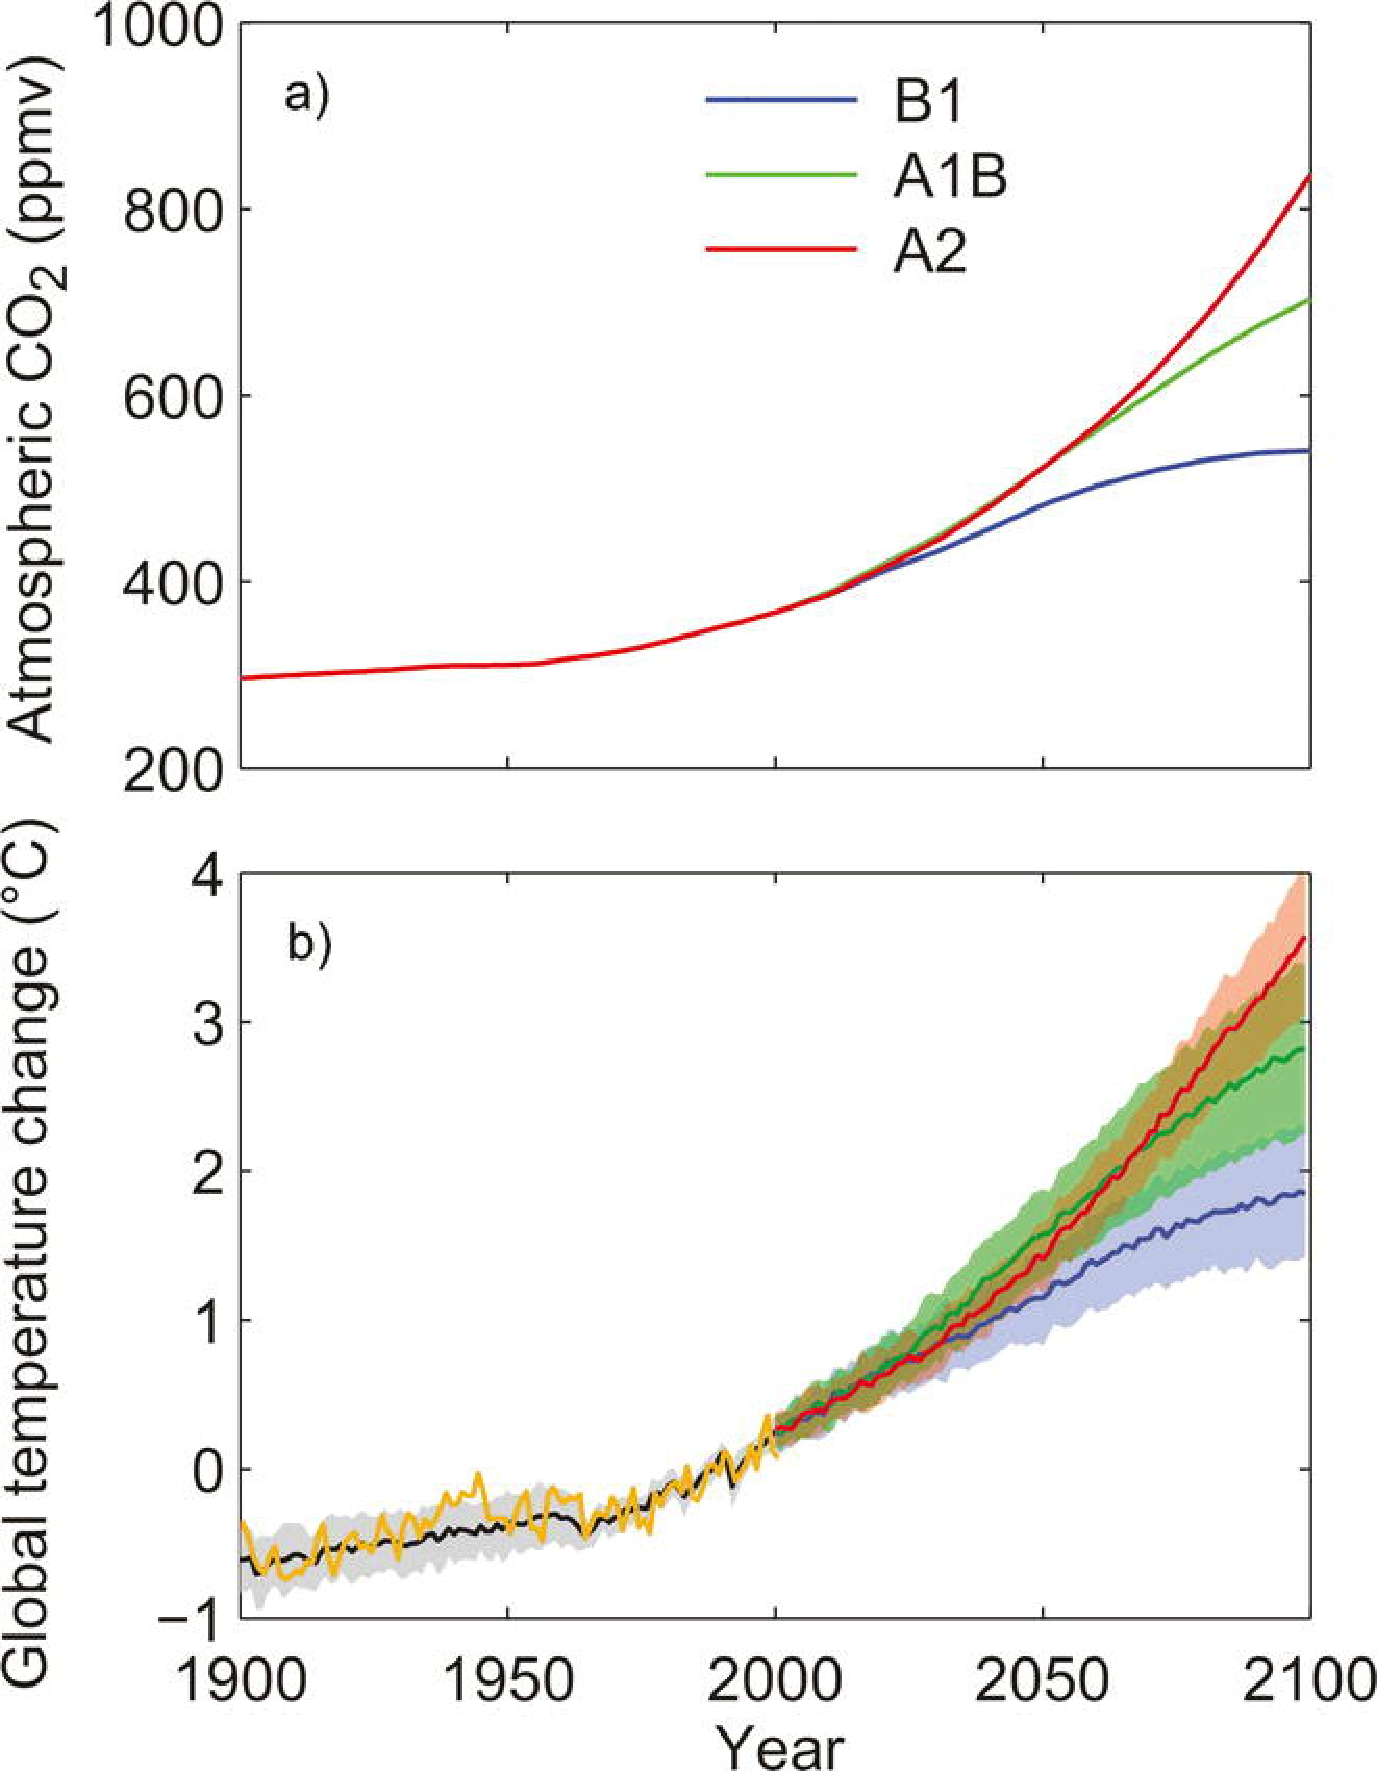
\includegraphics[width=19pc,angle=0]{figure01.pdf}\\
%\appendcaption{A1}{Caption here.}
%\end{figure}
%
% All appendix figures/tables should be placed in order AFTER the main figures/tables, i.e., tables, appendix tables, figures, appendix figures.
%
%%%%%%%%%%%%%%%%%%%%%%%%%%%%%%%%%%%%%%%%%%%%%%%%%%%%%%%%%%%%%%%%%%%%%
% REFERENCES
%%%%%%%%%%%%%%%%%%%%%%%%%%%%%%%%%%%%%%%%%%%%%%%%%%%%%%%%%%%%%%%%%%%%%
Make your BibTeX bibliography by using these commands:
\bibliographystyle{ametsoc2014}
\bibliography{paperpile}


%%%%%%%%%%%%%%%%%%%%%%%%%%%%%%%%%%%%%%%%%%%%%%%%%%%%%%%%%%%%%%%%%%%%%
% TABLES
%%%%%%%%%%%%%%%%%%%%%%%%%%%%%%%%%%%%%%%%%%%%%%%%%%%%%%%%%%%%%%%%%%%%%
%% enter tables at the end of the document, before figures.
%%
%
%\begin{table}[t]
%\caption{This is a sample table caption and table layout.  Enter as many tables as
%  necessary at the end of your manuscript. Table from Lorenz (1963).}\label{t1}
%\begin{center}
%\begin{tabular}{ccccrrcrc}
%\hline\hline
%$N$ & $X$ & $Y$ & $Z$\\
%\hline
% 0000 & 0000 & 0010 & 0000 \\
% 0005 & 0004 & 0012 & 0000 \\
% 0010 & 0009 & 0020 & 0000 \\
% 0015 & 0016 & 0036 & 0002 \\
% 0020 & 0030 & 0066 & 0007 \\
% 0025 & 0054 & 0115 & 0024 \\
%\hline
%\end{tabular}
%\end{center}
%\end{table}
\begin{table}[tb]
\caption{Control parameterization schemes used in numerical modelling configuration.}
\label{tab:WRFconfig}
\begin{center}
\begin{tabular}{cc}
\hline \hline
{\textbf{Parameterization}} & {\textbf{Scheme}} \\ \hline
{\textbf{Microphysics}} & Thompson \\ 
{\textbf{Longwave Radiation}} & RRTM  \\ 
{\textbf{Shortwave Radiation}} & Dudhia \\ 
{\textbf{Surface Layer}} & MYNN \\ 
{\textbf{Land Surface}} & Noah \\ 
{\textbf{Planetary Boundary Layer}} & MYNN Level 2.5  \\ 
\end{tabular}
\end{center}
\end{table}

\begin{table*}[tb]
\caption{Subjective summary of ensemble-member performance in each of the four ICBC experiments.}
\label{tab:summary}
\begin{center}
\begin{tabular}{c|cc}
\hline \hline
{\textbf{Date}} & {\textbf{Convection}} & {\textbf{Bowing}} \\ \hline
{\textbf{Case A: 26--27 May 2006}} & None & N/A \\
{\textbf{Case B:10--11 September 2009}} & All & Some  \\ 
{\textbf{Case C: 19--20 April 2011}} & All & Too weak \\ 
{\textbf{Case D: 15--16 August 2013}} & All & Most\\ 
\end{tabular}
\end{center}
\end{table*}

\begin{table}[tb]
\caption{Control parameterisation schemes used in numerical modelling configuration.}
\label{tab:MPs}
\begin{center}
\begin{tabular}{c}
Thompson \textdagger \\
WSM6 * \\
Kessler \\
Ferrier \\
WSM5 \\
WDM5 \\
Lin \\ 
WDM6 * \\
Morrison * \\
\hline \hline
\multicolumn{1}{l}{\textdagger \footnotesize{\qquad Control parameterisation}} \\
\multicolumn{1}{l}{*\footnotesize{\qquad Changed to be either hail- or graupel-like}} \\
\end{tabular}
\end{center}
\end{table}


%%%%%%%%%%%%%%%%%%%%%%%%%%%%%%%%%%%%%%%%%%%%%%%%%%%%%%%%%%%%%%%%%%%%%
% FIGURES
%%%%%%%%%%%%%%%%%%%%%%%%%%%%%%%%%%%%%%%%%%%%%%%%%%%%%%%%%%%%%%%%%%%%%
%% Enter figures at the end of the document, after tables.
%%
%
%\begin{figure}[htpb]
   %\centering
   %\subfloat[]{\label{fig:verif_2006}\includegraphics[width=19pc]{Images/verif_2006}}
   %\subfloat[]{\label{fig:verif_2009}\includegraphics[width=19pc]{Images/verif_2009}}\\
   %\subfloat[]{\label{fig:verif_2011}\includegraphics[width=19pc]{Images/verif_2011}}
   %\subfloat[]{\label{fig:verif_2013}\includegraphics[width=19pc]{Images/verif_2013}}\\
   %\caption{Radar reflectivity for the four cases found in this study: (a) a progressive bow echo, 0600 UTC, 27 May 2006; (b) a serial bow echo, 0800 UTC, 11 September 2009; (c) a serial bow echo, 0300 UTC, 20 May 2011; and (d) a progressive bow echo, 0300 UTC, 16 August 2013.}
   %\label{fig:verif_4panel}
%\end{figure}

\begin{figure}[tbph]
\centering
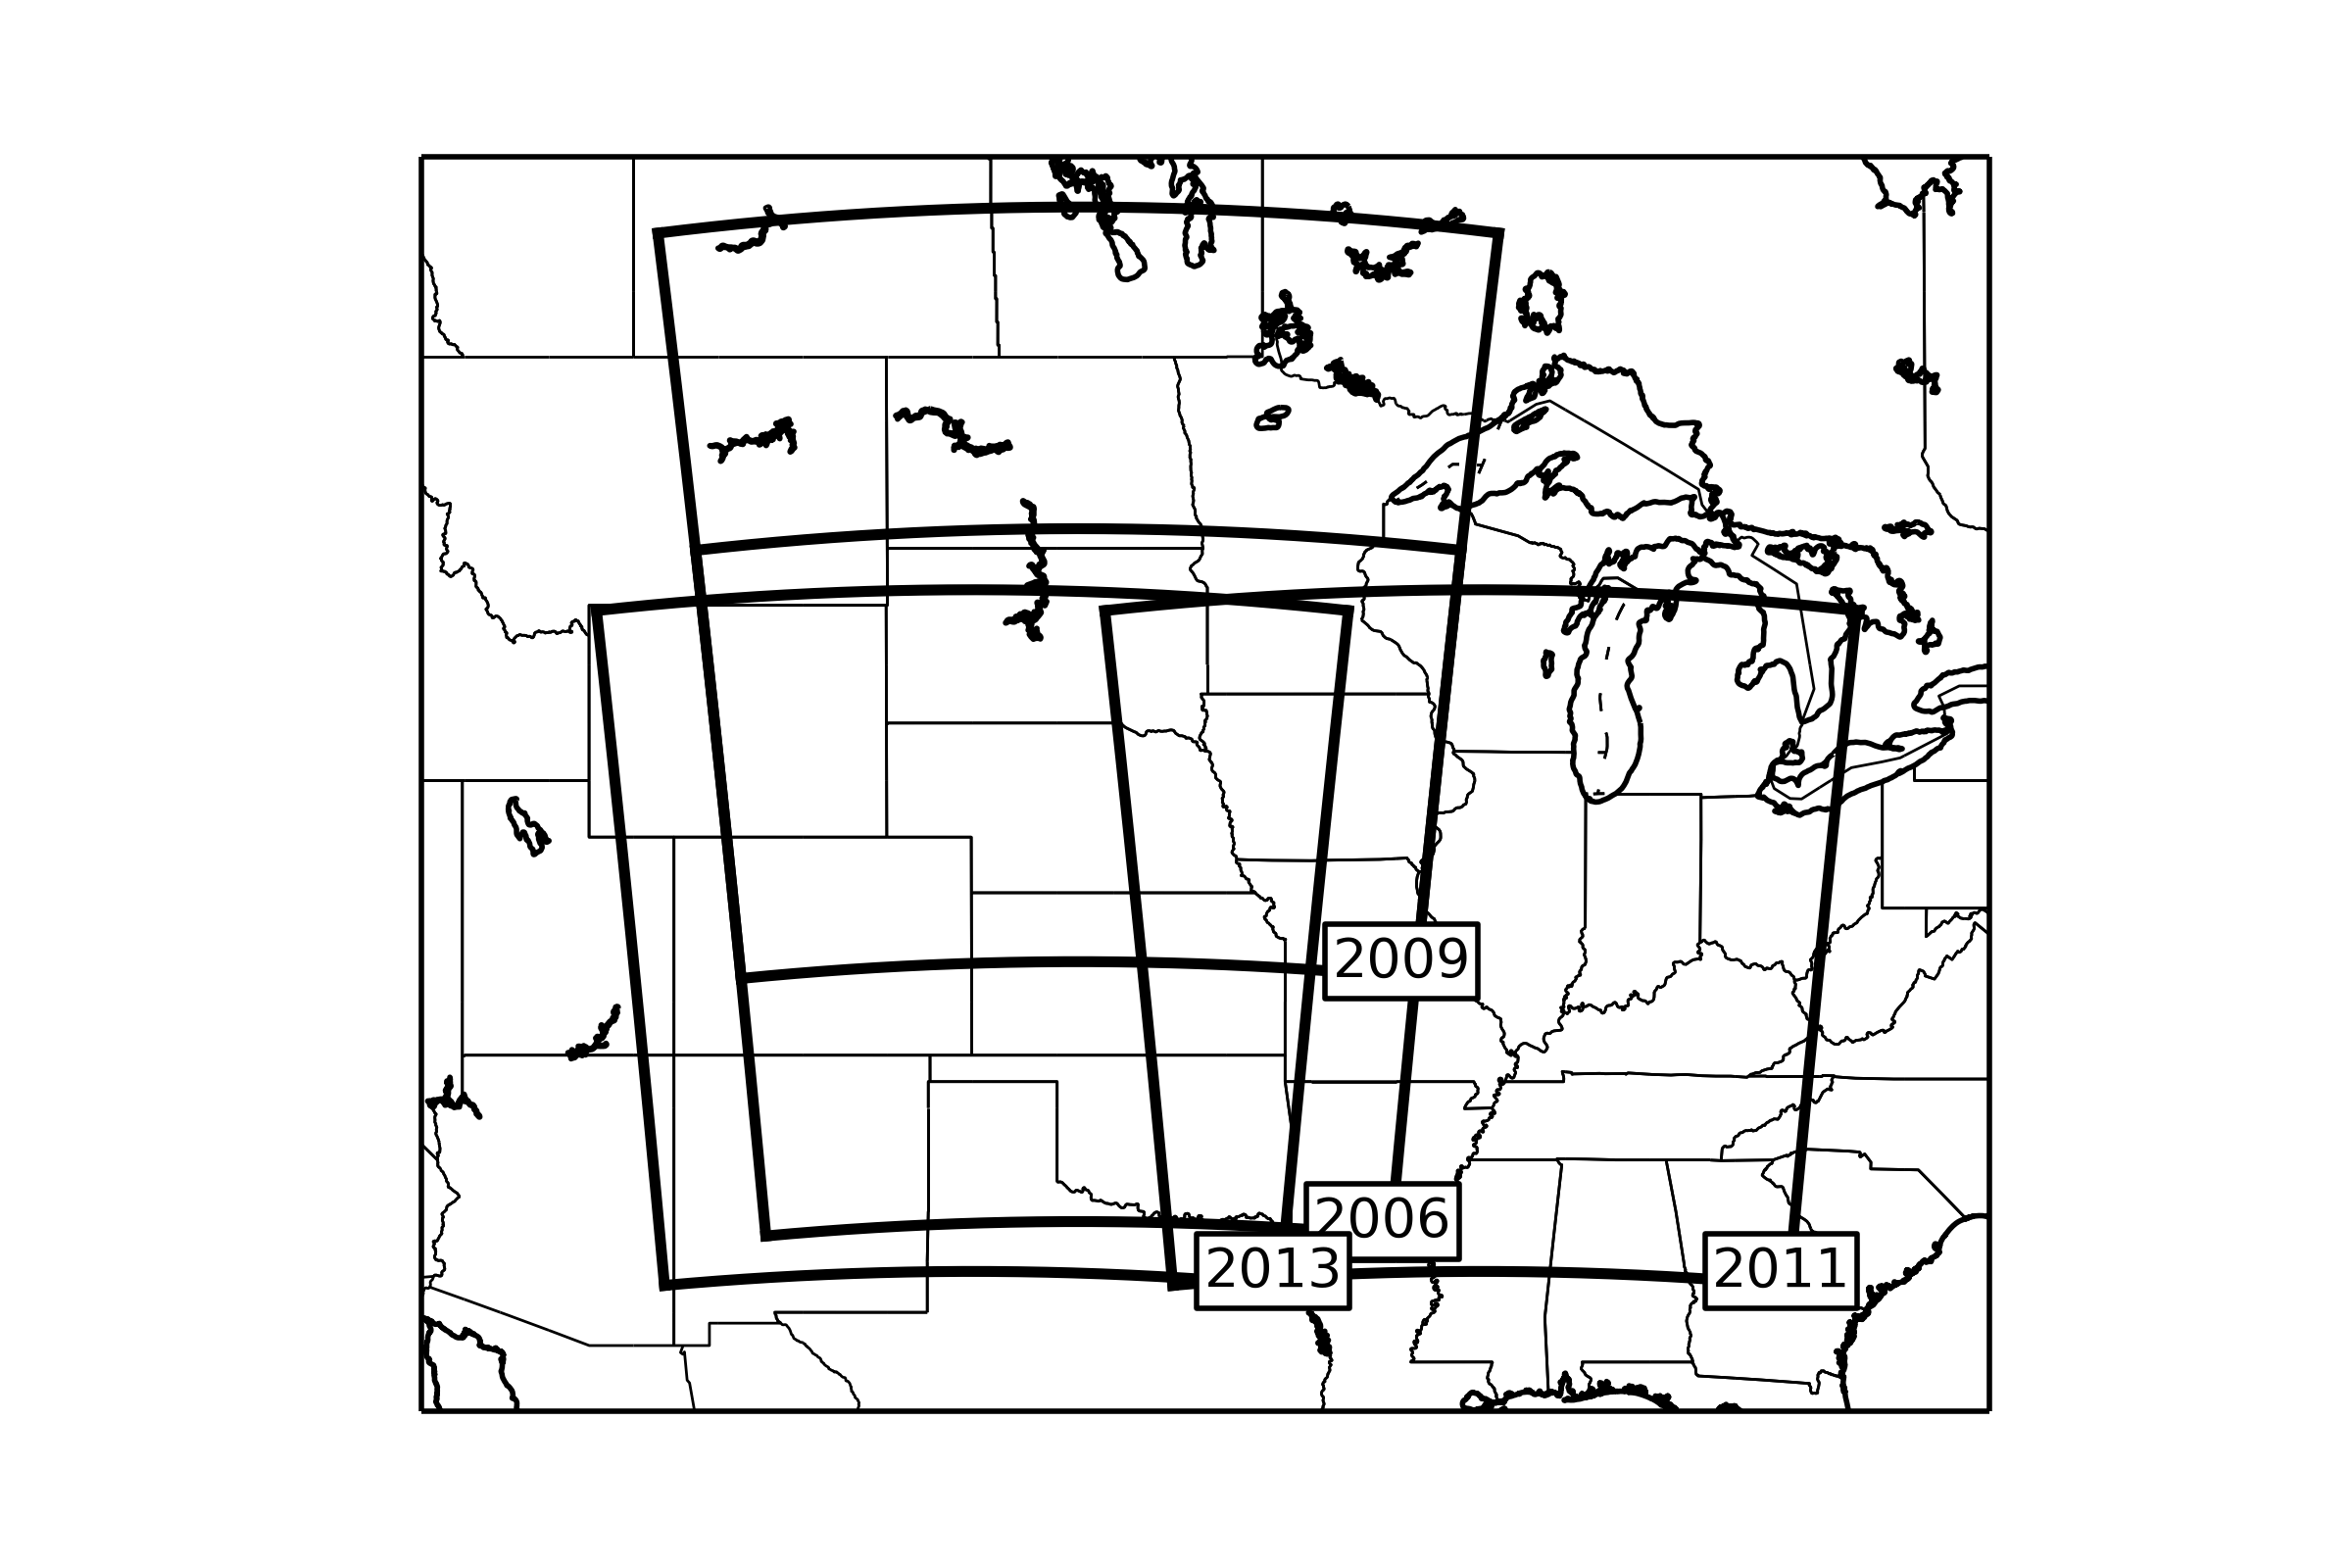
\includegraphics[width=21pc]{images/domains}
\caption{Domains for each of the four cases. Label denotes the year of each case (c.f. Fig~?.}
\label{fig:domains}
\end{figure}

%\begin{figure}[p]
%\centering
%\fbox{\includegraphics[width=0.88\textwidth]{Images/method}}
%\caption{Schematic of the methodology. From top to bottom, the ensemble experiments are termed ICBC, MXMP, and STCH. The example shown with arrows is for a method that follows the best-performing members in each preceding ensemble, to assess the stability of this `good' solution.}
%\label{fig:method}
%\end{figure}
%
%
%\begin{figure}[htpb]
   %\centering
   %\subfloat[Case A: 26--27 May 2006]{\label{fig:DTE_2006}\includegraphics[width=21pc]{Images/DTE_ICBC_Growth_Averages_2006}}
   %\subfloat[Case B: 10--11 September 2009]{\label{fig:DTE_2009}\includegraphics[width=21pc]{Images/DTE_ICBC_Growth_Averages_2009}}\\
   %\subfloat[Case C: 19--20 April 2011]{\label{fig:DTE_2011}\includegraphics[width=21pc]{Images/DTE_ICBC_Growth_Averages_2011}}
   %\subfloat[Case D: 15--16 August 2013]{\label{fig:DTE_2013}\includegraphics[width=21pc]{Images/DTE_ICBC_Growth_Averages_2013}}\\
   %\caption{Difference Total Energy (DTE, summed in three dimensions) growth with forecast time. Note the larger upper y-axis limit in (c).}
   %\label{fig:DTE_ICBC}
%\end{figure}
%
%
%\begin{figure}[htpb]
   %\centering
   %\subfloat[0300 UTC, 15 August]{\label{fig:DTE_1}\includegraphics[width=21pc]{Images/DTE_ICBC_p01}}
   %\subfloat[0900 UTC, 15 August]{\label{fig:DTE_2}\includegraphics[width=21pc]{Images/DTE_ICBC_p03}}\\
   %\subfloat[1800 UTC, 15 August]{\label{fig:DTE_3}\includegraphics[width=21pc]{Images/DTE_ICBC_p06}}
   %\subfloat[0600 UTC, 16 August]{\label{fig:DTE_4}\includegraphics[width=21pc]{Images/DTE_ICBC_p10}}\\
   %\caption{Difference Total Energy (DTE, summed with height) growth with forecast time, 15--16 August 2013.}
   %\label{fig:DTE_2D}
%\end{figure}
%
%\begin{figure}[htpb]
   %\centering
   %\subfloat[0300 UTC, 15 August]{\label{fig:DTE_1v}\includegraphics[width=19pc]{Images/cent_plains_201308150300}}\qquad
   %\subfloat[0900 UTC, 15 August]{\label{fig:DTE_2v}\includegraphics[width=19pc]{Images/cent_plains_201308150900}}\\ 
   %\subfloat[1800 UTC, 15 August]{\label{fig:DTE_3v}\includegraphics[width=19pc]{Images/cent_plains_201308151800}}\qquad
   %\subfloat[0600 UTC, 16 August]{\label{fig:DTE_4v}\includegraphics[width=19pc]{Images/cent_plains_201308160600}}\\ 
   %\caption{Observed composite radar reflectivity growth, at the same times as in Fig.~\ref{fig:DTE_2D}, 15--16 August 2013.}
   %\label{fig:verif}
%\end{figure}
%
%\begin{figure}[tbph]
%\centering
%\includegraphics[width=33pc]{Images/postage_ICBC_cref_sfc_201308160300}
%\caption{Postage-stamp plots of simulated composite reflectivity at 0300 UTC, 16 August 2013, for each of the ICBC ensemble members in Case D.}
%\label{fig:CaseD_ICBC}
%\end{figure}
%
%\begin{figure}[htpb]
   %\centering
   %\subfloat[ICBC]{\label{fig:DTE_ICBC2}\includegraphics[width=21pc]{Images/DTE_ICBC_Growth_Averages_2013}}
   %\subfloat[MXMP (p09 IC/BCs)]{\label{fig:DTE_MXMP}\includegraphics[width=21pc]{Images/DTE_MXMP_GEFS_p09_2013}}\\
   %\subfloat[STCH (p09, Thompson (control) microphysics)]{\label{fig:DTE_STCH_T}\includegraphics[width=21pc]{Images/DTE_STCH_GEFS_p09_2013_ICBC}}
    %\subfloat[STCH (p09, Morrison (hail-like) microphysics)]{\label{fig:DTE_STCH_M}\includegraphics[width=21pc]{Images/DTE_STCH_GEFS_p09_2013_Morrison_Hail}}\\
   %\caption{Difference Total Energy (DTE, summed in three dimensions) growth in various ensembles for Case D (15--16 August 2013).}
   %\label{fig:DTE_1D}
%\end{figure}
%
%
%\begin{figure}[tbph]
%\centering
%\includegraphics[width=33pc]{Images/postage_MXMP_cref_sfc_201308160300}
%\caption{As Fig.~\ref{fig:CaseD_ICBC}, but for MXMP ensemble members.}
%\label{fig:CaseD_MXMP}
%\end{figure}
%
%\begin{figure}[tbph]
%\centering
%\includegraphics[width=33pc]{Images/postage_STCH_cref_sfc_201308160300}
%\caption{As Fig.~\ref{fig:CaseD_ICBC}, but for STCH ensemble members.}
%\label{fig:CaseD_STCH}
%\end{figure}
%

%\begin{figure}[t]
%  \noindent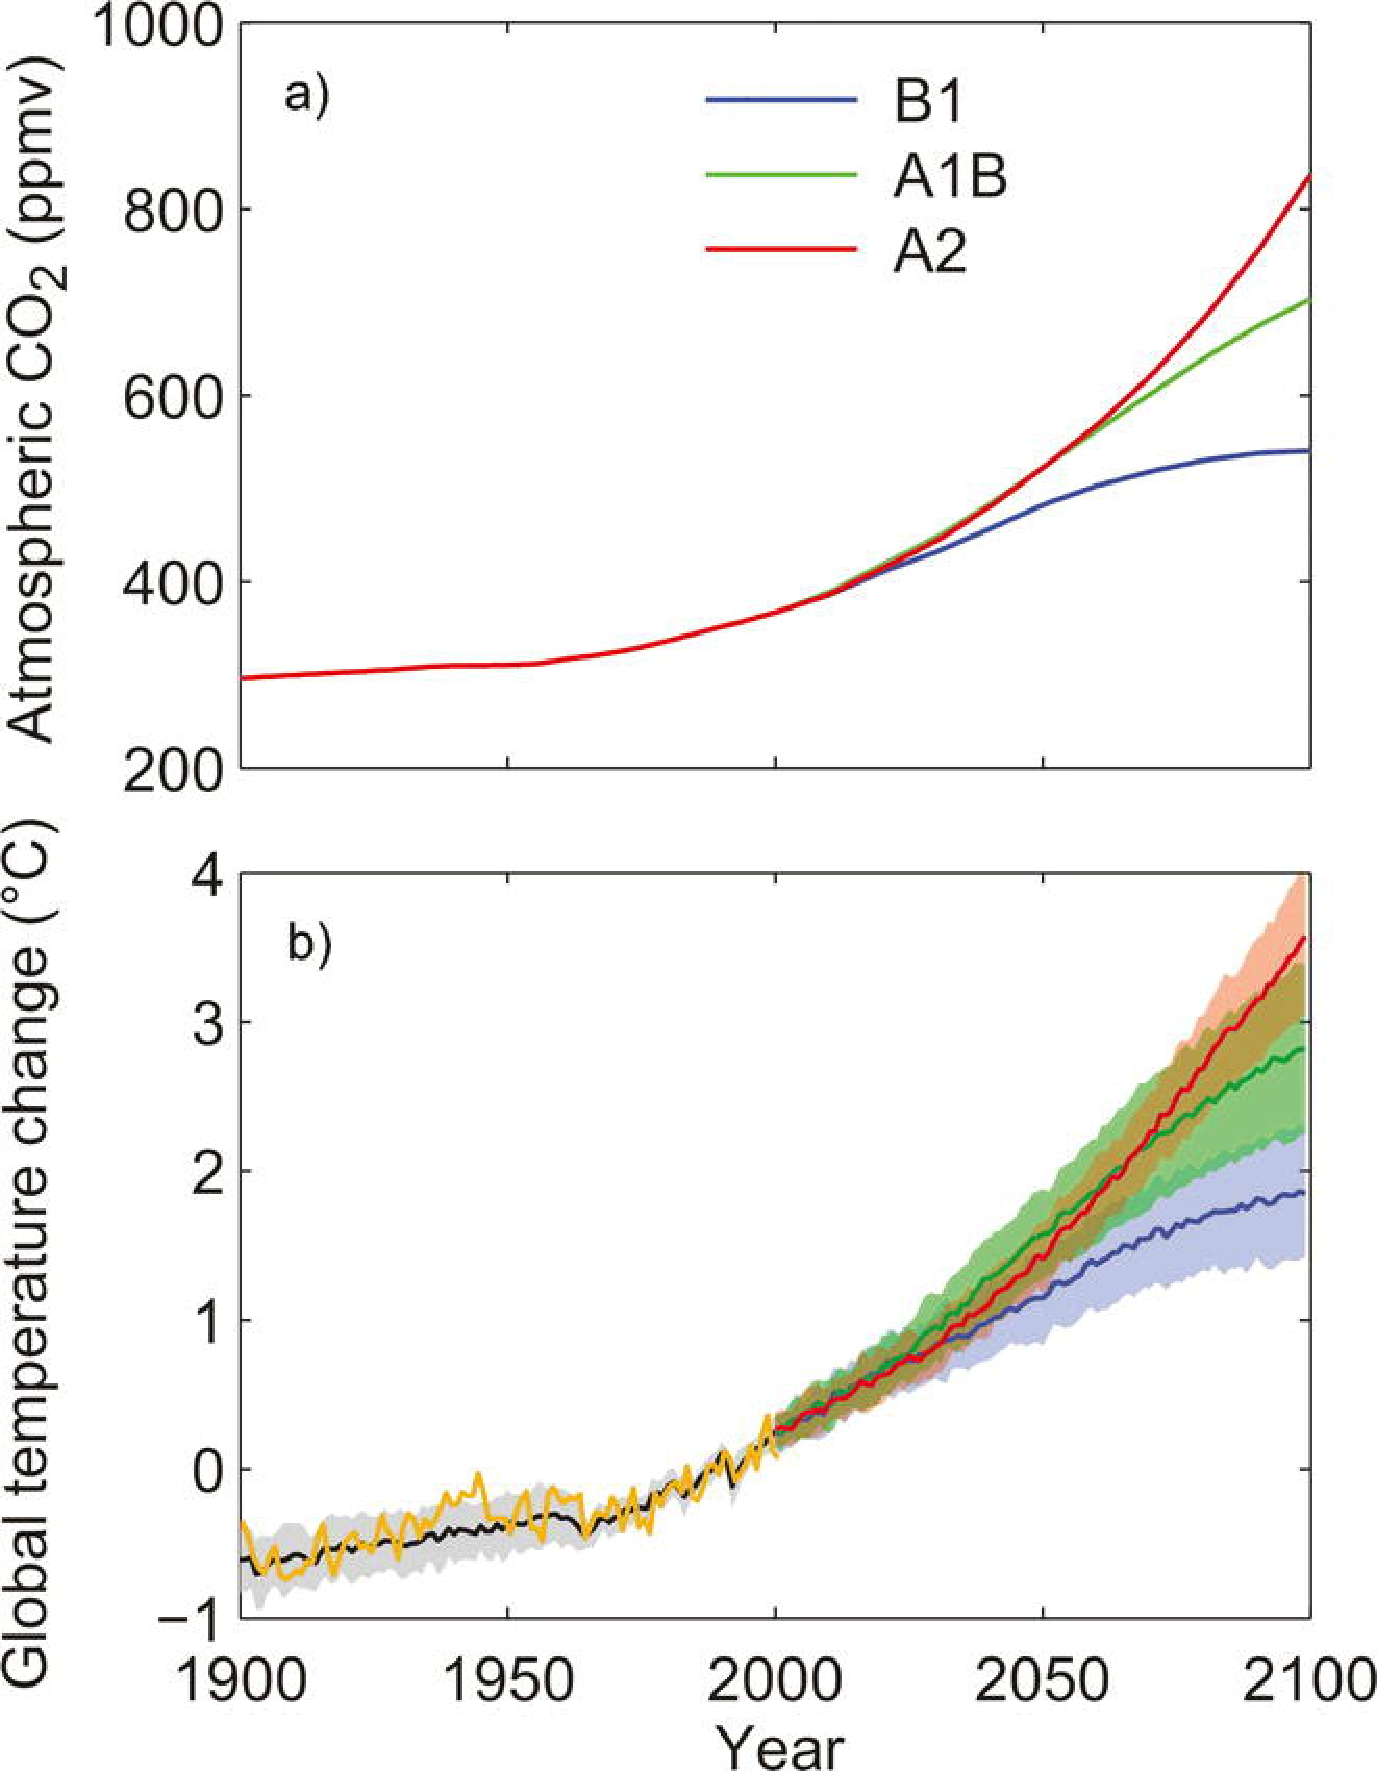
\includegraphics[width=19pc,angle=0]{figure01.pdf}\\
%  \caption{Enter the caption for your figure here.  Repeat as
%  necessary for each of your figures. Figure from \protect\cite{Knutti2008}.}\label{f1}
%\end{figure}

\end{document}
